\documentclass[aspectratio=169,11pt]{beamer}

\usepackage[utf8]{inputenc}
\usepackage[T1]{fontenc}
\usepackage{lmodern}
\usepackage{graphicx}
\usepackage{xcolor}
\usepackage{booktabs}
\usepackage{tabularx}
\usepackage{array}

\definecolor{navy}{HTML}{102A43}
\definecolor{blue}{HTML}{1F5F99}
\definecolor{teal}{HTML}{0F8B74}
\definecolor{muted}{HTML}{586B7C}
\definecolor{soft}{HTML}{F3F7FA}
\definecolor{line}{HTML}{D7E1EA}
\definecolor{finding}{HTML}{B83A2F}

\usetheme{default}
\setbeamertemplate{navigation symbols}{}
\setbeamercolor{normal text}{fg=navy,bg=white}
\setbeamercolor{structure}{fg=blue}
\setbeamercolor{frametitle}{fg=navy,bg=white}
\setbeamerfont{frametitle}{size=\Large,series=\bfseries}
\setbeamerfont{title}{size=\LARGE,series=\bfseries}
\setbeamerfont{subtitle}{size=\large}
\setbeamertemplate{frametitle}{\vspace{0.25em}\hspace{0.2em}\insertframetitle\par\vspace{0.10em}{\color{line}\rule{\textwidth}{0.5pt}}}
\setbeamertemplate{footline}{\hfill\color{muted}\scriptsize\insertframenumber/\inserttotalframenumber\hspace{0.8em}\vspace{0.35em}}
\setbeamertemplate{itemize item}{\color{teal}\raise0.2ex\hbox{\rule{0.7ex}{0.7ex}}}
\setbeamertemplate{itemize subitem}{\color{blue}\raise0.2ex\hbox{\rule{0.55ex}{0.55ex}}}

\newcommand{\code}[1]{\texttt{#1}}
\newcommand{\key}[1]{{\color{teal}\bfseries #1}}
\newcolumntype{Y}{>{\raggedright\arraybackslash}X}

\title{UVM Verification of a P4 Adder\\and a Windowed Register File}
\subtitle{RTL and post-synthesis functional verification}
\author{Erfan Taheri}
\date{}

\begin{document}

\begin{frame}[plain]
  \vfill
  \titlepage
  \vfill
\end{frame}

\begin{frame}{Verification scope}
\begin{columns}[T,onlytextwidth]
\column{0.48\textwidth}
  {\color{teal}\large\bfseries Registered P4 adder}\par\vspace{0.45em}
  \begin{itemize}
    \item 32-bit sparse-tree carry-select datapath
    \item fixed two-cycle latency
    \item carry propagation and prefix-tree activation
    \item complete RTL coverage and gate-level reuse
  \end{itemize}
\column{0.48\textwidth}
  {\color{teal}\large\bfseries Windowed register file}\par\vspace{0.45em}
  \begin{itemize}
    \item eight overlapping windows and eight globals
    \item 136 physical 64-bit registers
    \item stateful address translation and boundary control
    \item cycle-accurate reference model and RAL globals
  \end{itemize}
\end{columns}
\vspace{0.7em}
\centering
{\color{muted}Sequence-based stimulus, monitored transactions, independent prediction, and coverage-guided closure}
\end{frame}

\begin{frame}{P4 verification goal and checklist}
\key{Goal}\hspace{0.5em}Correct 33-bit arithmetic at the specified two-cycle latency, with direct evidence that the carry architecture was exercised.
\vspace{0.55em}

\begin{columns}[T,onlytextwidth]
\column{0.49\textwidth}
\begin{itemize}
  \item \textbf{Arithmetic}\quad \(\{C_{out},S\}=A+B+C_{in}\)
  \item \textbf{Timing}\quad operands at \(T\), result at \(T+2\)
  \item \textbf{Reset}\quad clear registers and flush invalid pipeline entries
\end{itemize}
\column{0.49\textwidth}
\begin{itemize}
  \item \textbf{Carry tree}\quad P, G, carry-in, and ripple in all eight blocks
  \item \textbf{Critical cases}\quad corners, full propagation, prefix terms
  \item \textbf{Reuse}\quad same checks and coverage after synthesis
\end{itemize}
\end{columns}
\end{frame}

\begin{frame}{P4 adder RTL and verification focus}
\centering
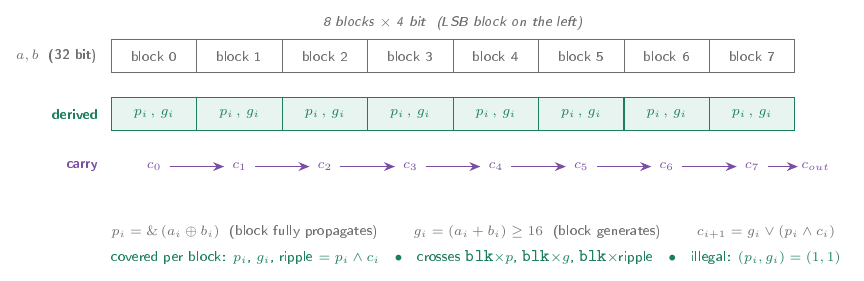
\includegraphics[width=0.95\textwidth]{../p4-adder/figures/coverage-model.png}
\vspace{0.45em}

\small
\begin{tabular}{@{}llll@{}}
\key{Pipeline} & \key{Arithmetic} & \key{Carry tree} & \key{Reset} \\
two-cycle alignment & independent 33-bit result & eight 4-bit blocks & registered wrapper
\end{tabular}
\end{frame}

\begin{frame}{P4 UVM environment}
\centering
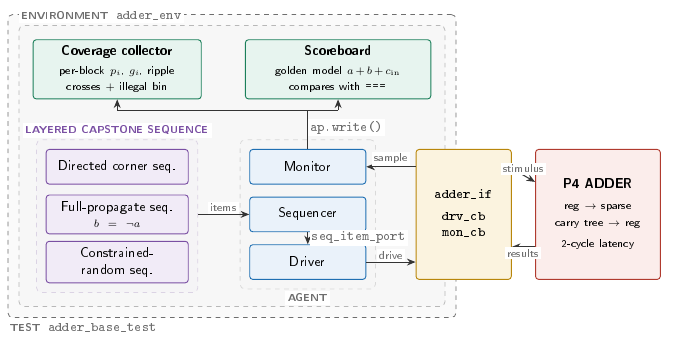
\includegraphics[height=0.76\textheight,keepaspectratio]{../p4-adder/figures/uvm-environment.png}
\end{frame}

\begin{frame}{P4 stimulus methodology}
\centering
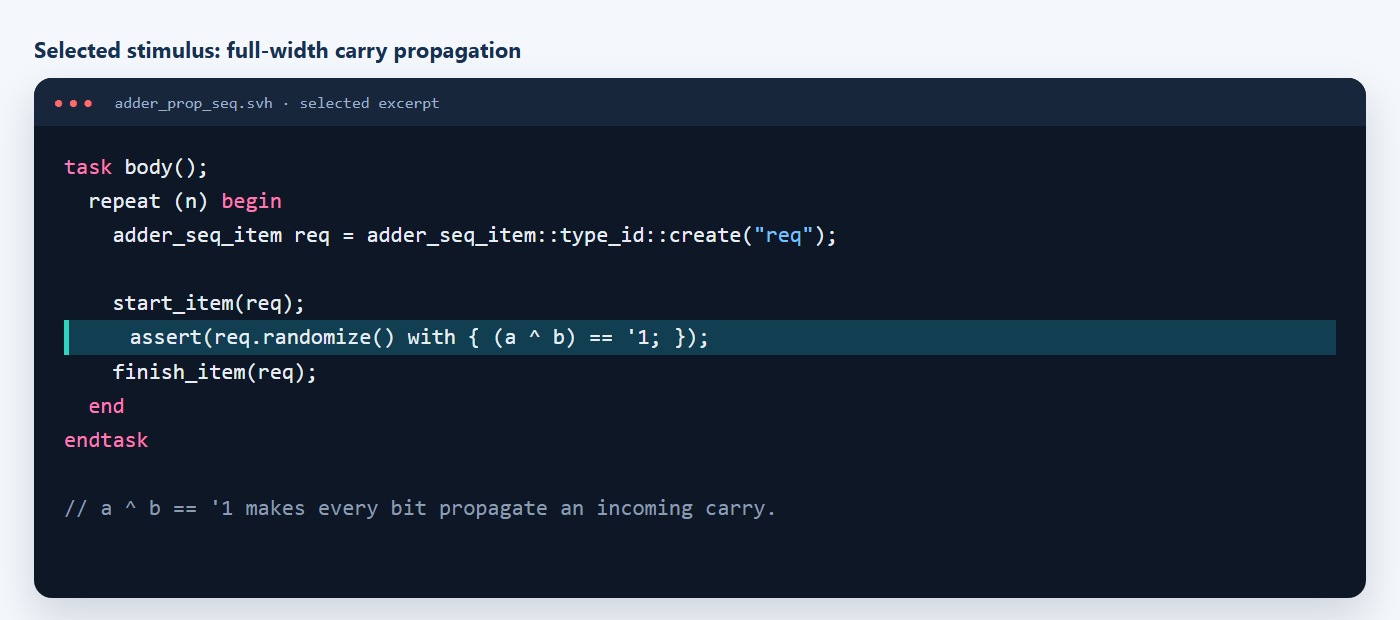
\includegraphics[width=0.80\textwidth]{../p4-adder/figures/full-propagation-sequence.png}
\vspace{0.4em}

\begin{columns}[T,onlytextwidth]
\column{0.48\textwidth}
\begin{itemize}
  \item directed arithmetic corners
  \item constrained-random operands
  \item full propagation with \(B=\lnot A\)
\end{itemize}
\column{0.48\textwidth}
\begin{itemize}
  \item non-masking prefix-tree vectors
  \item reset sequence for final closure
  \item pipeline drain before test completion
\end{itemize}
\end{columns}
\end{frame}

\begin{frame}{P4 functional coverage groups}
\centering
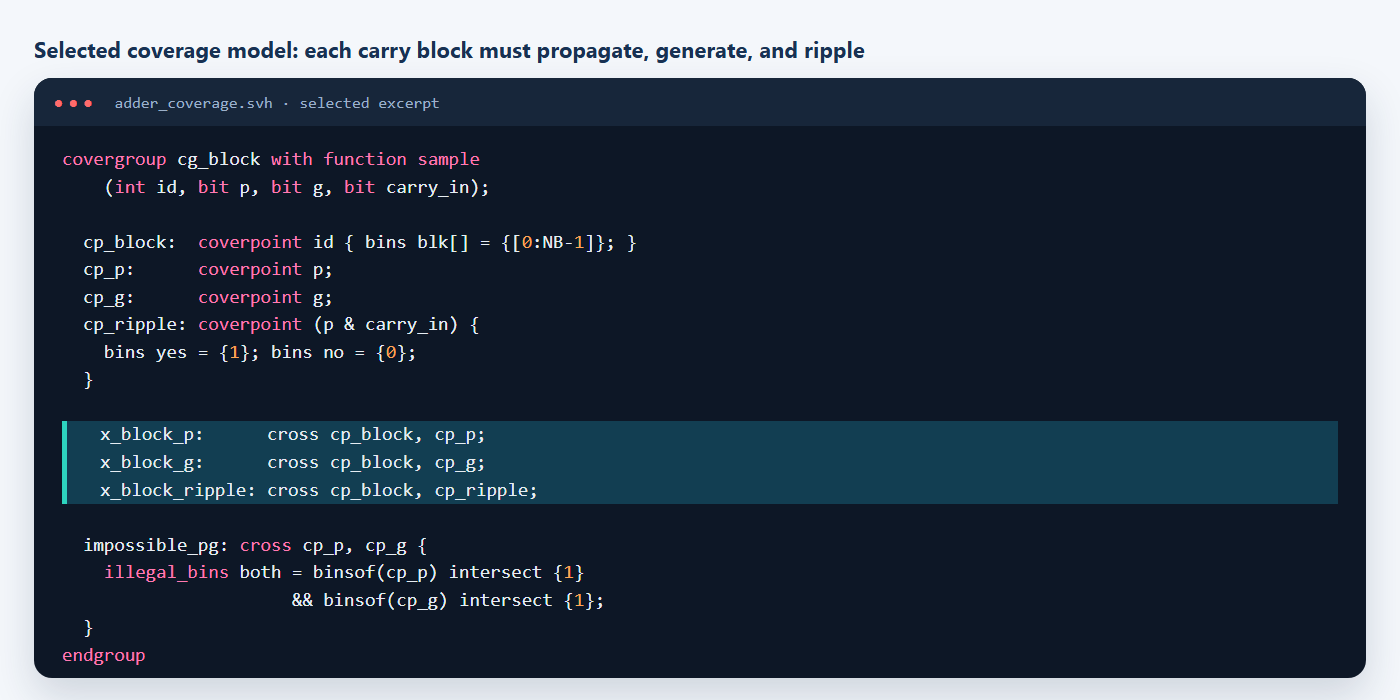
\includegraphics[width=0.68\textwidth]{../p4-adder/figures/coverage-bins.png}
\vspace{0.20em}

\begin{columns}[T,onlytextwidth]
\column{0.49\textwidth}
\key{Per 4-bit block}\quad index, propagate, generate, carry ripple
\column{0.49\textwidth}
\key{Crosses and top level}\quad block by condition, carry input/output, operand corners, full propagation
\end{columns}
\vspace{0.15em}
\centering
{\color{finding}Illegal state: \((P,G)=(1,1)\)}
\end{frame}

\begin{frame}{P4 coverage closure and results}
\begin{columns}[T,onlytextwidth]
\column{0.58\textwidth}
\small
\begin{tabularx}{\textwidth}{@{}Yr@{}}
\toprule
\textbf{Metric} & \textbf{Result} \\
\midrule
Scoreboard & 601 checks, 0 mismatches \\
Functional coverage & 100\% (117/117) \\
Statement coverage & 100\% \\
Branch coverage & 100\% \\
Expression coverage & 100\% \\
Toggle coverage & 100\% \\
Assertion coverage & 100\% (14/14) \\
Filtered RTL coverage & 100\% \\
Post-synth. functional & 100\% \\
\bottomrule
\end{tabularx}
\column{0.38\textwidth}
\key{Closure actions}\par\vspace{0.4em}
\begin{itemize}
  \item reset sequence closed the final RTL bins
  \item targeted vectors activated masked prefix terms
  \item unsigned range types corrected operand bins
  \item the same environment ran on the netlist
\end{itemize}
\end{columns}
\end{frame}

\begin{frame}{Register-file verification goal and checklist}
\key{Goal}\hspace{0.5em}Correct logical register mapping and window-management state on every clock, including the spill and fill boundaries.
\vspace{0.45em}

\begin{columns}[T,onlytextwidth]
\column{0.49\textwidth}
\begin{itemize}
  \item reset array, pointers, counters, and flags
  \item IN, LOCAL, OUT, and GLOBAL address mapping
  \item caller OUT to callee IN overlap
  \item registered reads and read-before-write
\end{itemize}
\column{0.49\textwidth}
\begin{itemize}
  \item call/return priority and disabled-state hold
  \item CWP, SWP, \code{CANSAVE}, and \code{CANRESTORE}
  \item spill/fill timing and boundary semantics
  \item RAL globals and mapped-netlist reuse
\end{itemize}
\end{columns}
\end{frame}

\begin{frame}{Windowed register file RTL}
\centering
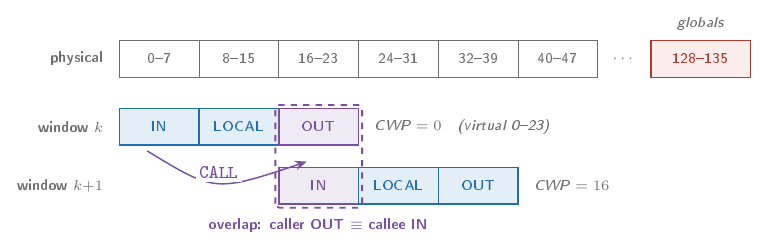
\includegraphics[width=0.91\textwidth]{../windowed-register-file/figures/window-overlap.png}
\vspace{0.45em}

\small
\begin{tabular}{@{}llll@{}}
\key{32 logical} & \key{136 physical} & \key{8 windows} & \key{8 globals} \\
IN/LOCAL/OUT/GLOBAL & 128 windowed + 8 fixed & 24 registers each & fixed mapping
\end{tabular}
\vspace{0.35em}

{\small \code{CALL}/\code{RET}\quad CWP/SWP\quad \code{SPILL}/\code{FILL}\\[0.15em]
\code{CANSAVE}/\code{CANRESTORE}}
\end{frame}

\begin{frame}{Windowed register-file UVM environment}
\centering
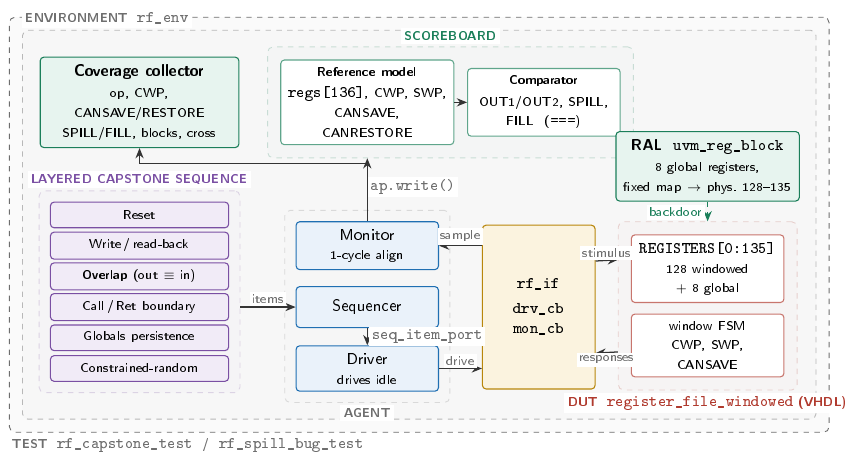
\includegraphics[height=0.76\textheight,keepaspectratio]{../windowed-register-file/figures/uvm-environment.png}
\end{frame}

\begin{frame}{Cycle-accurate transaction and timing model}
\begin{itemize}
  \item \key{One transaction equals one clock}\quad reset, call, return, access, or idle.
  \vspace{0.45em}
  \item \key{The driver applies an explicit idle}\quad one-shot controls never remain asserted while the sequencer is empty.
  \vspace{0.45em}
  \item \key{The monitor uses a one-entry pipeline}\quad inputs at cycle \(T\) are paired with registered outputs at \(T+1\).
  \vspace{0.45em}
  \item \key{The test drains the pipeline}\quad the final response reaches the scoreboard before the objection drops.
\end{itemize}
\end{frame}

\begin{frame}{Cycle-accurate reference model}
\begin{columns}[T,onlytextwidth]
\column{0.48\textwidth}
\key{State reproduced}\par\vspace{0.35em}
\begin{itemize}
  \item 136-entry physical register array
  \item CWP and SWP
  \item \code{CANSAVE} and \code{CANRESTORE}
  \item registered outputs and spill/fill pulses
\end{itemize}
\column{0.48\textwidth}
\key{Behavior reproduced}\par\vspace{0.35em}
\begin{itemize}
  \item logical-to-physical translation with wrap-around
  \item fixed mapping for global registers
  \item read-before-write ordering
  \item call/return priority and partial-reset behavior
\end{itemize}
\end{columns}
\vspace{0.65em}
\centering
The model advances once per monitored cycle and supplies CWP and counter state directly to coverage.
\end{frame}

\begin{frame}{Register-file sequences and overlap check}
\centering
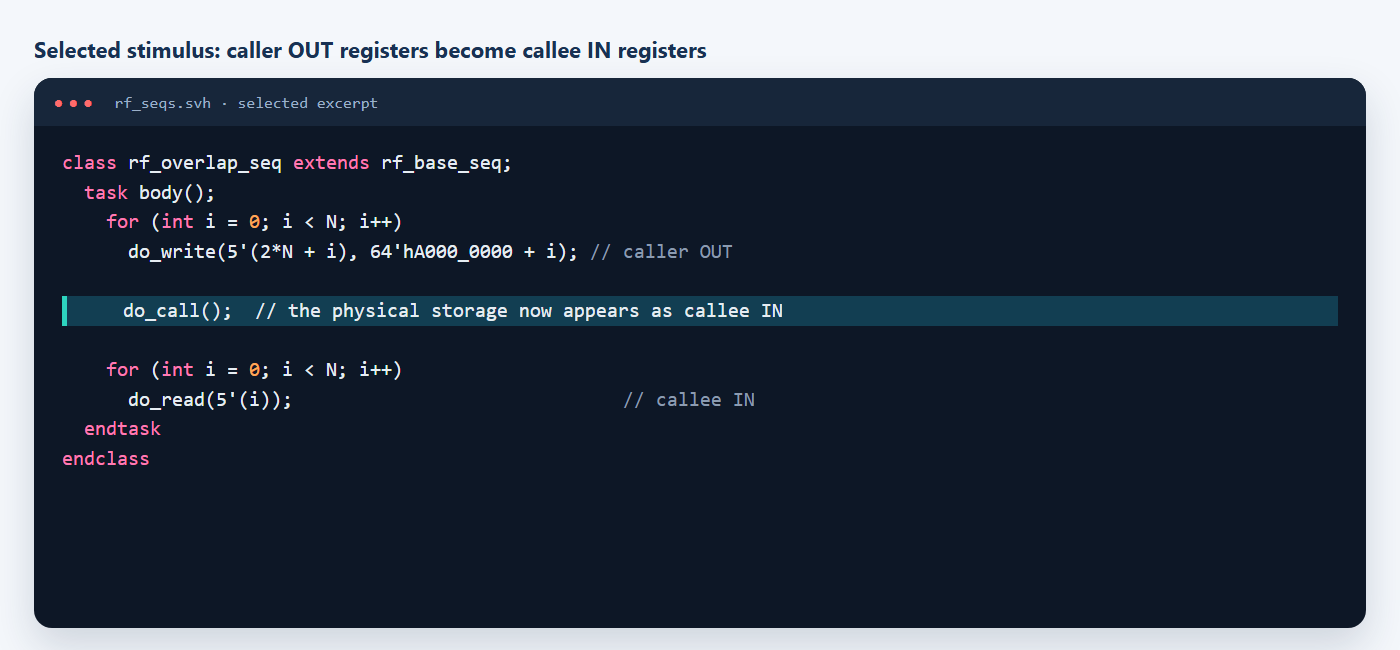
\includegraphics[width=0.75\textwidth]{../windowed-register-file/figures/overlap-sequence.png}
\vspace{0.20em}

\begin{columns}[T,onlytextwidth]
\column{0.49\textwidth}
\begin{itemize}
  \item write/read-back
  \item caller OUT to callee IN overlap
  \item globals across window changes
\end{itemize}
\column{0.49\textwidth}
\begin{itemize}
  \item repeated calls and returns to spill/fill
  \item constrained-random operations
  \item CWP sweep for coverage closure
\end{itemize}
\end{columns}
\end{frame}

\begin{frame}{Coverage of the internal FSM and counters}
\centering
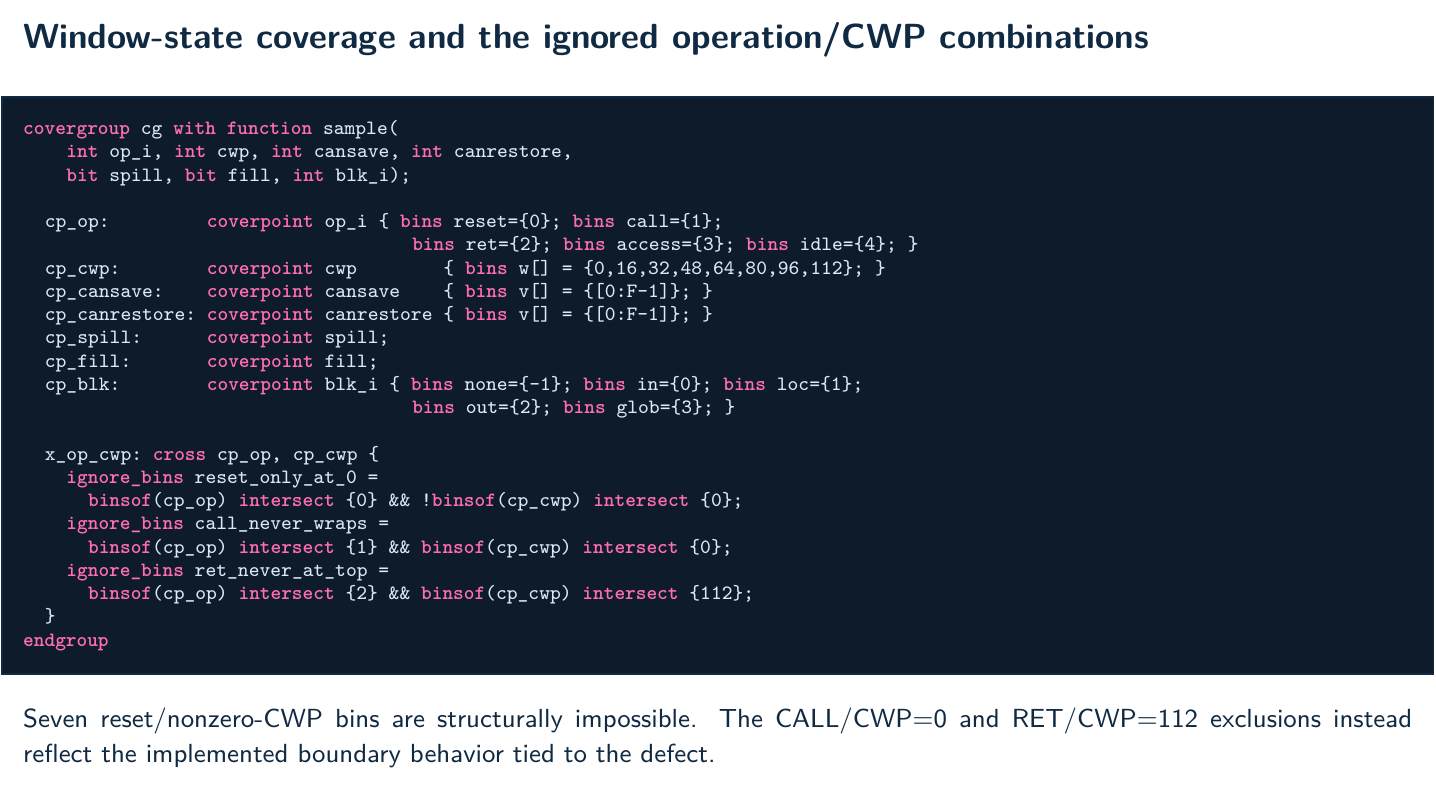
\includegraphics[width=0.77\textwidth]{../windowed-register-file/figures/coverage-bins.png}
\vspace{0.08em}

{\small
\key{Coverpoints:} operation, CWP, CANSAVE, CANRESTORE, SPILL, FILL, and addressed block.\\[0.15em]
\key{Cross:} every reachable operation at every reachable CWP position.}
\end{frame}

\begin{frame}{Functional coverage accounting}
\begin{columns}[T,onlytextwidth]
\column{0.34\textwidth}
\centering
{\color{teal}\Huge\bfseries 69/69}\par
{\color{muted}\large bins in the final covergroup}
\column{0.62\textwidth}
\key{The source contains three ignore-bin declarations}\par\vspace{0.30em}
\begin{itemize}
  \item seven reset/nonzero-CWP bins are structurally impossible
  \item CALL at sampled CWP 0 follows the faulty boundary path
  \item RET at sampled CWP 112 follows the mirrored path
\end{itemize}
\end{columns}
\vspace{0.45em}
The saved reports show only the resulting 69/69-bin model. No preserved report supports a separate pre-exclusion percentage.
\vspace{0.35em}

{\color{finding}\bfseries Only seven exclusions are inherently structural. Code coverage kept the two missed wrap assignments visible and exposed the defect.}
\end{frame}

\begin{frame}{RAL model and backdoor test}
\centering
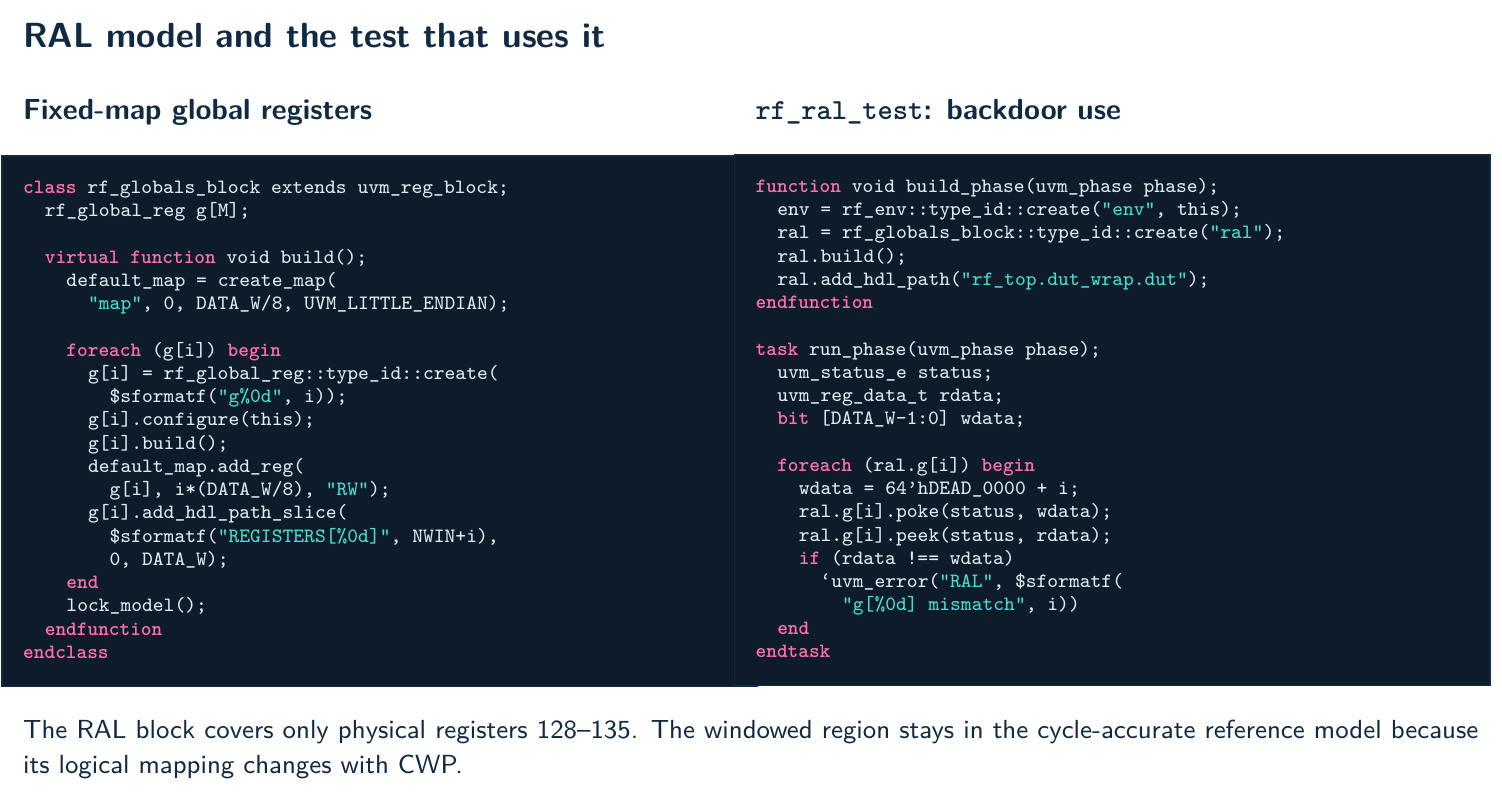
\includegraphics[width=0.94\textwidth]{../windowed-register-file/figures/ral-model-and-test.png}
\end{frame}

\begin{frame}{Windowed register-file results}
\small
\centering
\begin{tabularx}{0.86\textwidth}{@{}Xr@{}}
\toprule
\textbf{Metric} & \textbf{Result} \\
\midrule
Scoreboard & 1,058 checks, 0 mismatches \\
Functional coverage & 100\% (69/69) \\
Statement coverage & 94.73\% (36/38) \\
Branch coverage & 94.59\% (35/37) \\
Toggle coverage & 100\% (438/438) \\
Assertion coverage & 100\% \\
Filtered overall RTL coverage & 97.86\% \\
Post-synthesis functional coverage & 100\% (69/69) \\
Timing & 3.00 ns, slack 1.36 ns \\
\bottomrule
\end{tabularx}
\par
\vspace{0.55em}
\textbf{Code coverage exposed the defect:} the only misses were the two CWP wrap assignments at the spill/fill boundary.
\end{frame}

\begin{frame}{Directed confirmation of the code-coverage finding}
\centering
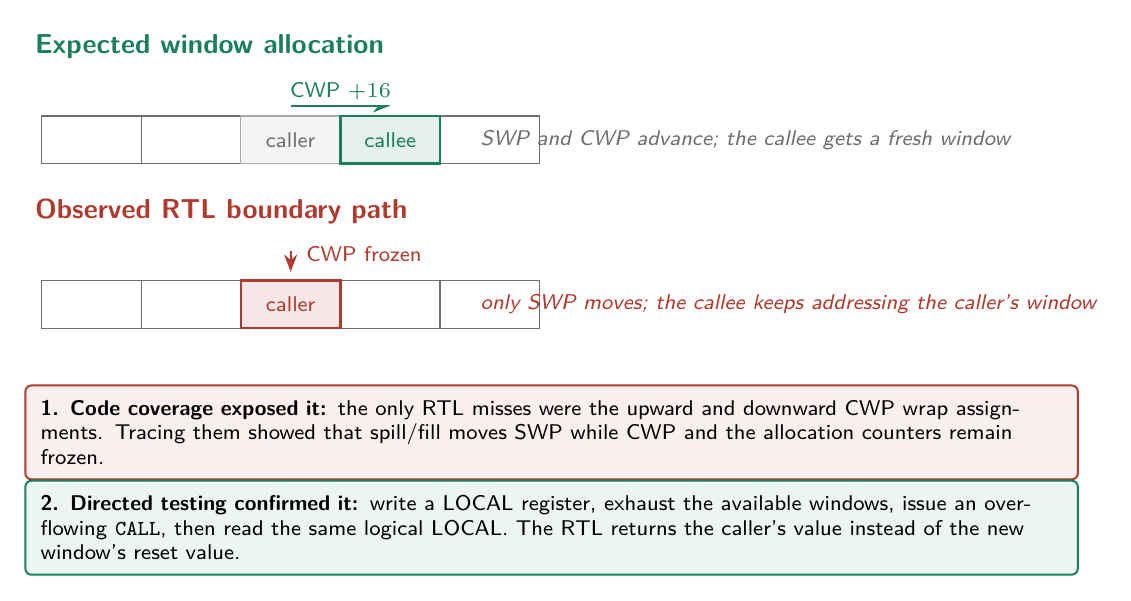
\includegraphics[width=0.72\textwidth]{../windowed-register-file/figures/overflow-finding.png}
\vspace{0.12em}

{\small\color{finding}\bfseries The missed wrap lines led to the frozen CWP/counter path; the specification-oriented LOCAL test then confirmed reuse of the caller's window.}
\end{frame}

\begin{frame}{Post-synthesis findings}
\begin{columns}[T,onlytextwidth]
\column{0.48\textwidth}
\key{Window-state reset}\par\vspace{0.35em}
One mapped \code{CANRESTORE} bit could remain unknown after power-up under synchronous-only reset logic. The spill path worked while fill became unknown.

\vspace{0.45em}
An asynchronous reset on the small control state removes the ambiguity.
\column{0.48\textwidth}
\key{Four-state monitoring}\par\vspace{0.35em}
Two-state response fields converted a sampled \code{x} to zero before it reached the scoreboard.

\vspace{0.45em}
DUT-sampled fields were changed to \code{logic}, preserving unknowns for strict comparison.
\end{columns}
\vspace{0.7em}
\centering
Both issues were invisible in the RTL regression and appeared only at gate level.
\end{frame}

\begin{frame}{Summary and learning resources}
\begin{columns}[T,onlytextwidth]
\column{0.48\textwidth}
\key{P4 adder}\par
Complete RTL coverage, 117/117 functional bins, independent arithmetic prediction, and unchanged gate-level reuse.

\vspace{0.65em}
\key{Windowed register file}\par
Stateful reference model, internal FSM and counter coverage, 69/69 functional bins, RAL globals, and boundary-defect analysis.
\column{0.48\textwidth}
\key{Learning resources}\par\vspace{0.35em}
\begin{itemize}
  \item Ray Salemi, \emph{UVM and SystemVerilog training course}, Siemens
  \item Ashok B. Mehta, \emph{ASIC/SoC Functional Design Verification: A Comprehensive Guide to Technologies and Methodologies}
\end{itemize}
\end{columns}
\end{frame}

\end{document}
